\documentclass[12pt,a4paper]{article}
\usepackage[utf8]{inputenc}
\usepackage{amssymb, amsmath, multicol}
\usepackage[russian]{babel}
\usepackage{graphicx}
\usepackage[shortcuts,cyremdash]{extdash}
\usepackage{wrapfig}
\usepackage{floatflt}
\usepackage{lipsum}
\usepackage{concmath}
\usepackage{euler}
\usepackage{tikz}  
\usetikzlibrary{graphs}

\oddsidemargin=-15.4mm
\textwidth=190mm
\headheight=-32.4mm     
\textheight=277mm
\tolerance=100
\parindent=0pt
\parskip=8pt
\pagestyle{empty}
\renewcommand{\tg}{\mathop{\mathrm{tg}}\nolimits}
\renewcommand{\ctg}{\mathop{\mathrm{ctg}}\nolimits}
\renewcommand{\arctan}{\mathop{\mathrm{arctg}}\nolimits}
\newcommand{\divisible}{\mathop{\raisebox{-2pt}{\vdots}}}

\graphicspath{{pictures/}}

\begin{document}
	\begin{center}
		Лабораторная работа 2.4.1 \\
		"Определение теплоты испарения жидкости" \\
		Б01-005 Радькин Кирилл
	\end{center}
	
	Цель работы:
	
	\begin{itemize}
		\item Измерение давления насыщенного пара жидкости при разной температуре
		\item вычисление по полученным данным теплоты испарения с помощью уравнения Клапейрона–Клаузиуса	
	\end{itemize}
	
	В работе используются:
	
	\begin{itemize}
		\item Термостат; герметический сосуд, заполненный исследуемой жидкостью; отсчетный микроскоп
	\end{itemize}
	
	Испарением называется переход вещества из жидкого в газообразное состояние. Оно происходит на свободной поверхности жидкости. При испарении с поверхности вылетают молекулы, образуя над ней пар. Для выхода из жидкости молекулы должны преодолеть силы молекулярного сцепления. Кроме того, при испарении совершается работа против внешнего давления $P$ , поскольку объем жидкости меньше объема пара. Не все молекулы жидкости способны совершить эту работу, а только те из них, которые обладают достаточной кинетической энергией. Поэтому переход части молекул в пар приводит к обеднению жидкости быстрыми молекулами, т. е. к ее охлаждению. Чтобы испарение проходило без изменения температуры, к жидкости нужно подводить тепло. Количество теплоты, необходимое для изотермического испарения одного моля жидкости при внешнем давлении, равном упругости ее насыщенных паров, называется молярной теплотой испарения (парообразования).\\
	
Теплоту парообразования жидкостей можно измерить непосредственно при помощи калориметра. Такой метод, однако, не позволяет получить точных результатов из-за неконтролируемых потерь тепла, которые трудно сделать малыми. В настоящей работе для определения теплоты испарения применен косвенный метод, основанный на формуле Клапейрона–Клаузиуса:

	\begin{equation}
		\dfrac{dP}{dT} = \dfrac{L}{T(V_2 - V_1)}
	\end{equation}
	
Здесь $P$ — давление насыщенного пара жидкости при температуре $T$ , $T$ — абсолютная температура жидкости и пара, $L$ — теплота испарения жидкости, $V_2$ — объем пара, $V_1$ — объем жидкости. Найдя из опыта $\dfrac{dP}{dT}$ , $T$, $V_2$ и $V_1$ , можно определить $L$ путем расчета. Величины $L$, $V_2$ и $V_1$ в формуле (1) должны относиться к одному и тому
же количеству вещества; мы будем относить их к одному молю. \\

В нашем приборе измерения производятся при давлениях ниже атмосферного. В этом случае задача существенно упрощается.\\

В таблице для ряда жидкостей приведены: температура, при которой давление насыщенных паров равно атмосферному, величины $V_2$ и $V_1$ , входящие в (1), а также константы $a$ и $b$ в уравнении Ван-дер-Ваальса.

	\begin{tabular}{| c | c | c | c | c | c |} \hline
		 Вещество & $T_k$, K & $V_1, 10^{-6}$, м$^3$/моль & $V_2, 10^{-3}$, м$^3$/моль & $b, 10^{-6}$ м$^3$/моль & $a$, Па $\cdot$ м$^6$ \\ \hline
		 Вода & $373$ & $18$ & $31$ & $26$ & $0.4$ \\ 
		 $CCl_4$ & $350$ & $97$ & $29$ & $126$ & $1.95$ \\
		 Этиловый эфир & $307$ & $104$ & $25$ & $137$ & $1.8$ \\
		 Этиловый спирт & $351$ & $58$ & $29$ & $84$ & $1.2$ \\ \hline
	\end{tabular}
	
	Из таблицы видно, что $V_1$ не превосходит $0,5\%$ от $V_2$ . При нашей точности опытов величиной $V_1$ в (1) можно пренебречь. Обратимся теперь к $V_2$ , которое в дальнейшем будем обозначать просто $V$ . Объем $V$ связан с давлением и температурой уравнением Ван-дер-Ваальса:
	
	
	\begin{equation}
		\left( P + \dfrac{a}{V^2} \right) \left( V - b \right) = RT
	\end{equation}
	
	Из рассмотрения таблицы следует, что $b$ одного порядка с $V_1$. В уравнении Ван-дер-Ваальса величиной b следует пренебречь. Пренебрежение членом $\dfrac{a}{V_2}$ по сравнению с $P$ вносит ошибку менее $3\%$. При давлении ниже атмосферного ошибки становятся еще меньше. Таким образом, при давлениях ниже атмосферного уравнение Ван-дер-Вааль-са для насыщенного пара мало отличается от уравнения Клапейрона. Положим поэтому:
	
	\begin{equation}
		V = \dfrac{RT}{P}
	\end{equation}
	
	Подставляя (3) в (1), пренебрегая $V_1$ и разрешая уравнение относительно $L$, найдем:
	
	\begin{equation}
		L = \dfrac{RT^2}{P} \dfrac{dP}{dT} = -R \dfrac{d \left( \ln P \right))}{d \left( 1/T \right)}
	\end{equation}
	
	Эта формула является окончательной. В нашем опыте температура жидкости измеряется термометром, давление пара определяется при помощи манометра, а производные $dP/dT$ или $d(\ln P)/d(1/T)$ находятся графически как угловой коэффициент касательной к кривой $P(T)$ или соответственно к кривой, у которой по оси абсцисс отложено $1/T$ , а по оси ординат $\ln P$. \\
	
	Экспериментальная установка:
	
	\begin{center}
		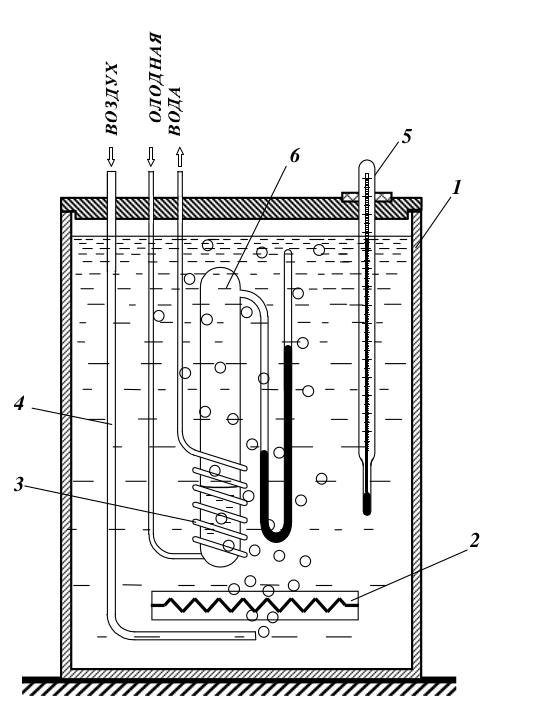
\includegraphics[scale=0.4]{pic1.png}
	\end{center}
	
	Схема установки изображена на рисунке. Наполненный водой резервуар 1 играет роль термостата. Нагревание термостата производится спиралью 2, подогревае-
мой электрическим током. Для охлаждения воды в термостате через змеевик 3. Схема установки для определения теплоты пропускается водопроводная вода. Вода испарения в термостате перемешивается воздухом, поступающим через трубку 4. Температура воды измеряется термометром 5. В термостат погружен запаянный прибор 6 с исследуемой жидкостью. Над ней находится насыщенный пар (перед заполнением прибора воздух из него был откачан). Давление насыщенного пара определяется по ртутному манометру, соединенному с исследуемым объемом. Отсчет показаний манометра производится при помощи микроскопа. \\

Описание прибора указывает на второе важное преимущество предложенного косвенного метода измерения $L$ перед прямым. При непосредственном измерении теплоты испарения опыты нужно производить при неизменном давлении, и прибор не может быть запаян. При этом невозможно обеспечить такую чистоту и неизменность экспериментальных условий, как при нашей постановке опыта. \\

Описываемый прибор обладает важным недостатком: термометр определяет температуру термостата, а не исследуемой жидкости (или ее пара). Эти температуры близки друг к другу лишь в том случае, если нагревание происходит достаточно медленно. Убедиться в том, что темп нагревания не является слишком быстрым, можно, сравнивая результаты, полученные при нагревании и при остывании прибора. Такое сравнение необходимо сделать. Для ориентировки укажем, что температуру воды в калориметре следует менять не быстрее, чем на $1^\circ C$ в течение 1–3 минут.  

	\begin{center}
		Ход работы:
	\end{center}
	
	\begin{enumerate}
		\item Будем измерять разность уровней в ртутном U-образном манометре с помощью микроскопа и температуру по термометру.
		\item Включим термостат.При работе через каждый градус измеряем давление и температуру. Продолжаем повышать температуру в течение половины имеющегося у нас времени, чтобы успеть произвести измерения при остывании прибора.\\
		
			\begin{tabular}{| c | c | c | c | c | c | c | c | c | c | c |} \hline
				$T^\circ C$ & $21$ & $22$ & $23$ & $24$ & $25$ & $26$ & $27$ & $28$ & $29$ & $30$ \\ \hline
				$h_b, mm$ & $91.6$ & $92.25$ & $92.65$ & $93.50$ & $94.35$ & $95.25$ & $95.65$ & $96.55$ & $96.9$ & $98.25$ \\ \hline
				
				$h_m, mm$ & $74.9$ & $73.45$ & $72.35$ & $71.45$ & $71.00$ & $70.45$ & $69.35$ & $69.25$ & $67.65$ & $67.50$ \\ \hline
			\end{tabular}				
			
			\begin{tabular}{| c | c | c | c | c | c |} \hline
				$T^\circ C$ & $31$ & $32$ & $33$ & $34$ & $35$ \\ \hline
				$h_b, mm$ & $99.00$ & $99.45$ & $100.95$ & $101.95$ & $103.85$ \\ \hline
				$h_m, mm$ & $66.40$ & $65.65$ & $64.60$ & $63.85$ & $63.35$ \\ \hline
			\end{tabular}
			
		\item Проведите те же измерения при охлаждении жидкости. Установите такой поток воды, чтобы охлаждение шло примерно тем же темпом, что и нагревание.\\
		
			\begin{tabular}{| c | c | c | c | c | c | c | c | c | c | c |} \hline
				$T^\circ C$ & $35$ & $34$ & $33$ & $32$ & $31$ & $30$ & $29$ & $28$ & $27$ & $26$ \\ \hline
				$h_b, mm$ & $103.85$ & $102.35$ & $101.80$ & $101.25$ & $100.15$ & $99.25$ & $98.00$ & $96.75$ & $96.50$ & $95.75$ \\ \hline
				
				$h_m, mm$ & $63.35$ & $63.75$ & $64.55$ & $65.65$ & $66.65$ & $67.85$ & $68.60$ & $68.95$ & $70.00$ & $71.00$ \\ \hline
			\end{tabular}				
			
			\begin{tabular}{| c | c | c | c | c | c |} \hline
				$T^\circ C$ & $25$ & $24$ & $23$ & $22$ & $21$ \\ \hline
				$h_b, mm$ & $94.60$ & $93.85$ & $92.95$ & $92.40$ & $92.35$ \\ \hline
				$h_m, mm$ & $70.65$ & $71.75$ & $72.65$ & $72.85$ & $73.65$ \\ \hline
			\end{tabular}
			
		\item Построим графики $P$ от $T$, $\ln P$ от $1 / T$ ($P$ вычислим по формуле $P = \rho g h; \rho = 13600 kg/m^3, g = 9.81 m/c^2, h = h_b - h_m$:	
		
		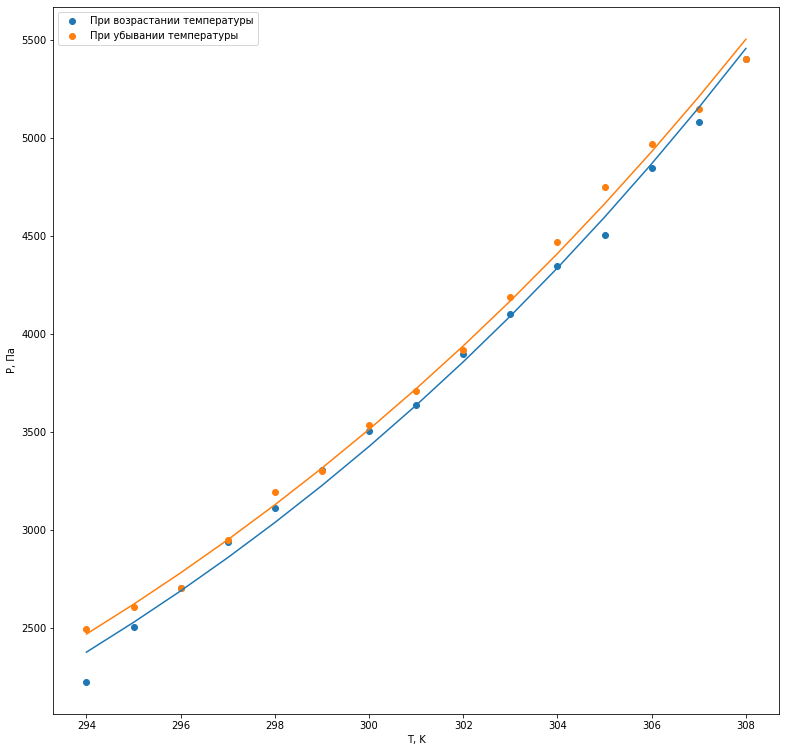
\includegraphics[scale=0.6]{pic2.png} \\
		
		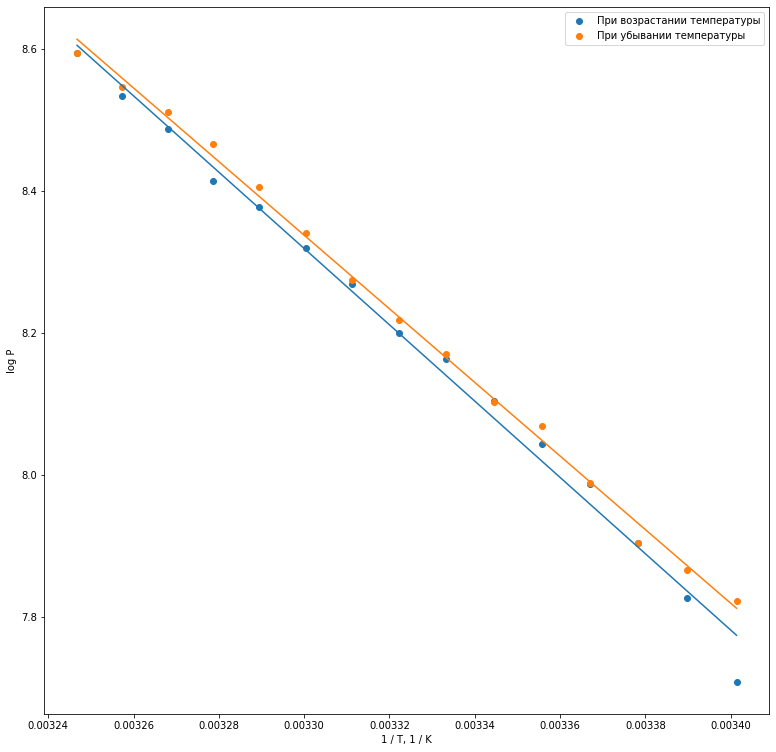
\includegraphics[scale=0.6]{pic3.png} \\
		
		\item Вычислим $L$ (молярную):
			\begin{itemize}
				\item При нагревании: $L = 44651 \pm 1022$ Дж/моль
				\item При охлаждении: $L = 43069 \pm 573$ Дж/моль
			\end{itemize}
			
		Табличное значение: $L = 40660$ Дж/моль
	\end{enumerate}
	
	Вывод: полученные нами значения достаточно близки друг к другу и к табличному значению, ошибка составляет порядка $\sim 9\%$. Оцененная нами ошибка измерений составляет $\sim 2\%$.
\end{document}
